\documentclass[conference]{IEEEtran}
\usepackage{cite}
\usepackage{amsmath,amssymb,amsfonts}
\usepackage{algorithmic}
\usepackage{graphicx}
\usepackage{textcomp}
\usepackage{xcolor}
\usepackage{placeins}
\def\BibTeX{{\rm B\kern-.05em{\sc i\kern-.025em b}\kern-.08em
    T\kern-.1667em\lower.7ex\hbox{E}\kern-.125emX}}

\title{A Study on NSL-KDD Dataset for Network Security}
\author{\IEEEauthorblockN{Rojina Deuja}
\IEEEauthorblockA{\textit{Department of Computer Science and Engineering} \\
\textit{University of Nebraska-Lincoln}\\
Lincoln, United States \\
rojinadeuja33g@gmail.com}}
\date{November 2020}

\begin{document}

\maketitle

\begin{abstract}
Network Security is an ever-expanding and highly demanding research areas in the field of Information Technology. Intrusion detection is the task of monitoring various events that occur in a computer system or a communication network, and analyzing them for signs of intrusions. The NSL-KDD dataset is a benchmark dataset used to design and evaluate various intrusion detection systems. In this paper, we analyze various parameters that characterize a network system and design a model to identify vulnerable systems.
\end{abstract}

\begin{IEEEkeywords}
networks, Intrusion Detection Systems, NSL-KDD, classification
\end{IEEEkeywords}

\section{Introduction}
Network Security is an ever-expanding and highly demanding research areas in the field of Information Technology. Network security is primarily concerned with implementing a set of rules, configurations or systems that are designed to enhance the protection of critical data in any communication network. Whether it be a home network or a business network, there is always the chance of the system could be exploited if not properly secured. An established network security system can help prevent the loss, theft or unauthorized access of sensitive information.

An intrusion is an attempt to compromise the Confidentiality, Integrity and Availability (CIA), or to bypass the security mechanisms of a computer or network \cite{b1}. Intrusion detection is the task of monitoring various events that occur in a computer system or a communication network, and analyzing them for signs of intrusions. Intrusion detection methodologies are generally classified into three main categories: Signature-based Detection (SD), Anomaly-based Detection (AD) and Stateful Protocol Analysis (SPA). Anomaly-based Detection (AD), also known as Behavior-based Detection identifies anomalous events in the network system. An anomaly is any event that deviates from normal/known behavior. These anomalies can be identified by monitoring or evaluation regular activities, connections, hosts or users in the network over a period of time \cite{b2}.

\section{Dataset}
NSL-KDD dataset was released as a new and improved version of KDD'99 dataset by the University of New Brunswick. It is used as a benchmark data to evaluate various intrusion detection methods on modern-day network systems.
The dataset contains of four different subsets: KDDTrain+, KDDTest+, KDDTrain+\_20Percentand KDDTest+\_20Percent. The first two subsets contain all of the train and test sets while the latter subsets contain only 20\% of the train and test sets respectively.
For the purpose of this experiment, we will use the KDDTrain+ and KDDTest+ datasets and refer to them as train and test sets respectively.
The dataset consists of internet traffic records encountered by a real Intrusion Detection System.

There are 43 attributes in total, where 42 are the input features, \emph{Score} is an field denoting the difficulty level and a binary class \emph{attack} that classifies if there has been any attack on the traffic input.

\section{Intrusion Detection}
There are various techniques that can be applied for Intrusion Detection. Liao et al. \cite{b2} identify three subclasses of intrusion detection methodologies: Signature-based Detection (SD), Anomaly-based Detection (AD) and Stateful Protocol Analysis (SPA). For our intrusion detection task, we will use a Signature-based Detection technique. A signature can be described as a pattern that denotes a known attack or threat. Signature-base Detection is used to identify such patterns by comparing them against normal or expected behavior. Since the knowledge gathered from prior attacks and system vulnerabilities are utilized to find more possibly harmful behavior, SD is also known as Knowledge-based Detection or Misuse Detection. It is one of the simplest and most effective method to detect any forms of anticipated attacks.

\section{Exploratory Data Analysis}
We carry out various data analysis tasks on the NSL-KDD dataset in order to help us understand the data better. There are 43 columns in the dataset, out of which the `attack' field contains the type of attacks detected in the network. There are 22 different types of attacks and a \emph{normal} value for no attack. The types of network attacks and their occurrence in the dataset is shown in Table \ref{tab1}. The most common types of attacks can be seen in the chart shown in Fig \ref{fig1}.

\begin{table}[htbp]
\caption{Types of Network Attacks}
\begin{center}
\begin{tabular}{|c|c|}
\hline
Type of Attack & Count \\
\hline
normal (None)	&	67342	\\
neptune	&	41214	\\
satan	&	3633	\\
ipsweep	&	3599	\\
portsweep	&	2931	\\
smurf	&	2646	\\
nmap	&	1493	\\
back	&	956	\\
teardrop	&	892	\\
warezclient	&	890	\\
pod	&	201	\\
guess\_passwd	&	53	\\
buffer\_overflow	&	30	\\
warezmaster	&	20	\\
land	&	18	\\
imap	&	11	\\
rootkit	&	10	\\
loadmodule	&	9	\\
ftp\_write	&	8	\\
multihop	&	7	\\
phf	&	4	\\
perl	&	3	\\
spy	&	2	\\
\hline
\end{tabular}
\label{tab1}
\end{center}
\end{table}

\begin{figure}[htbp]
\centerline{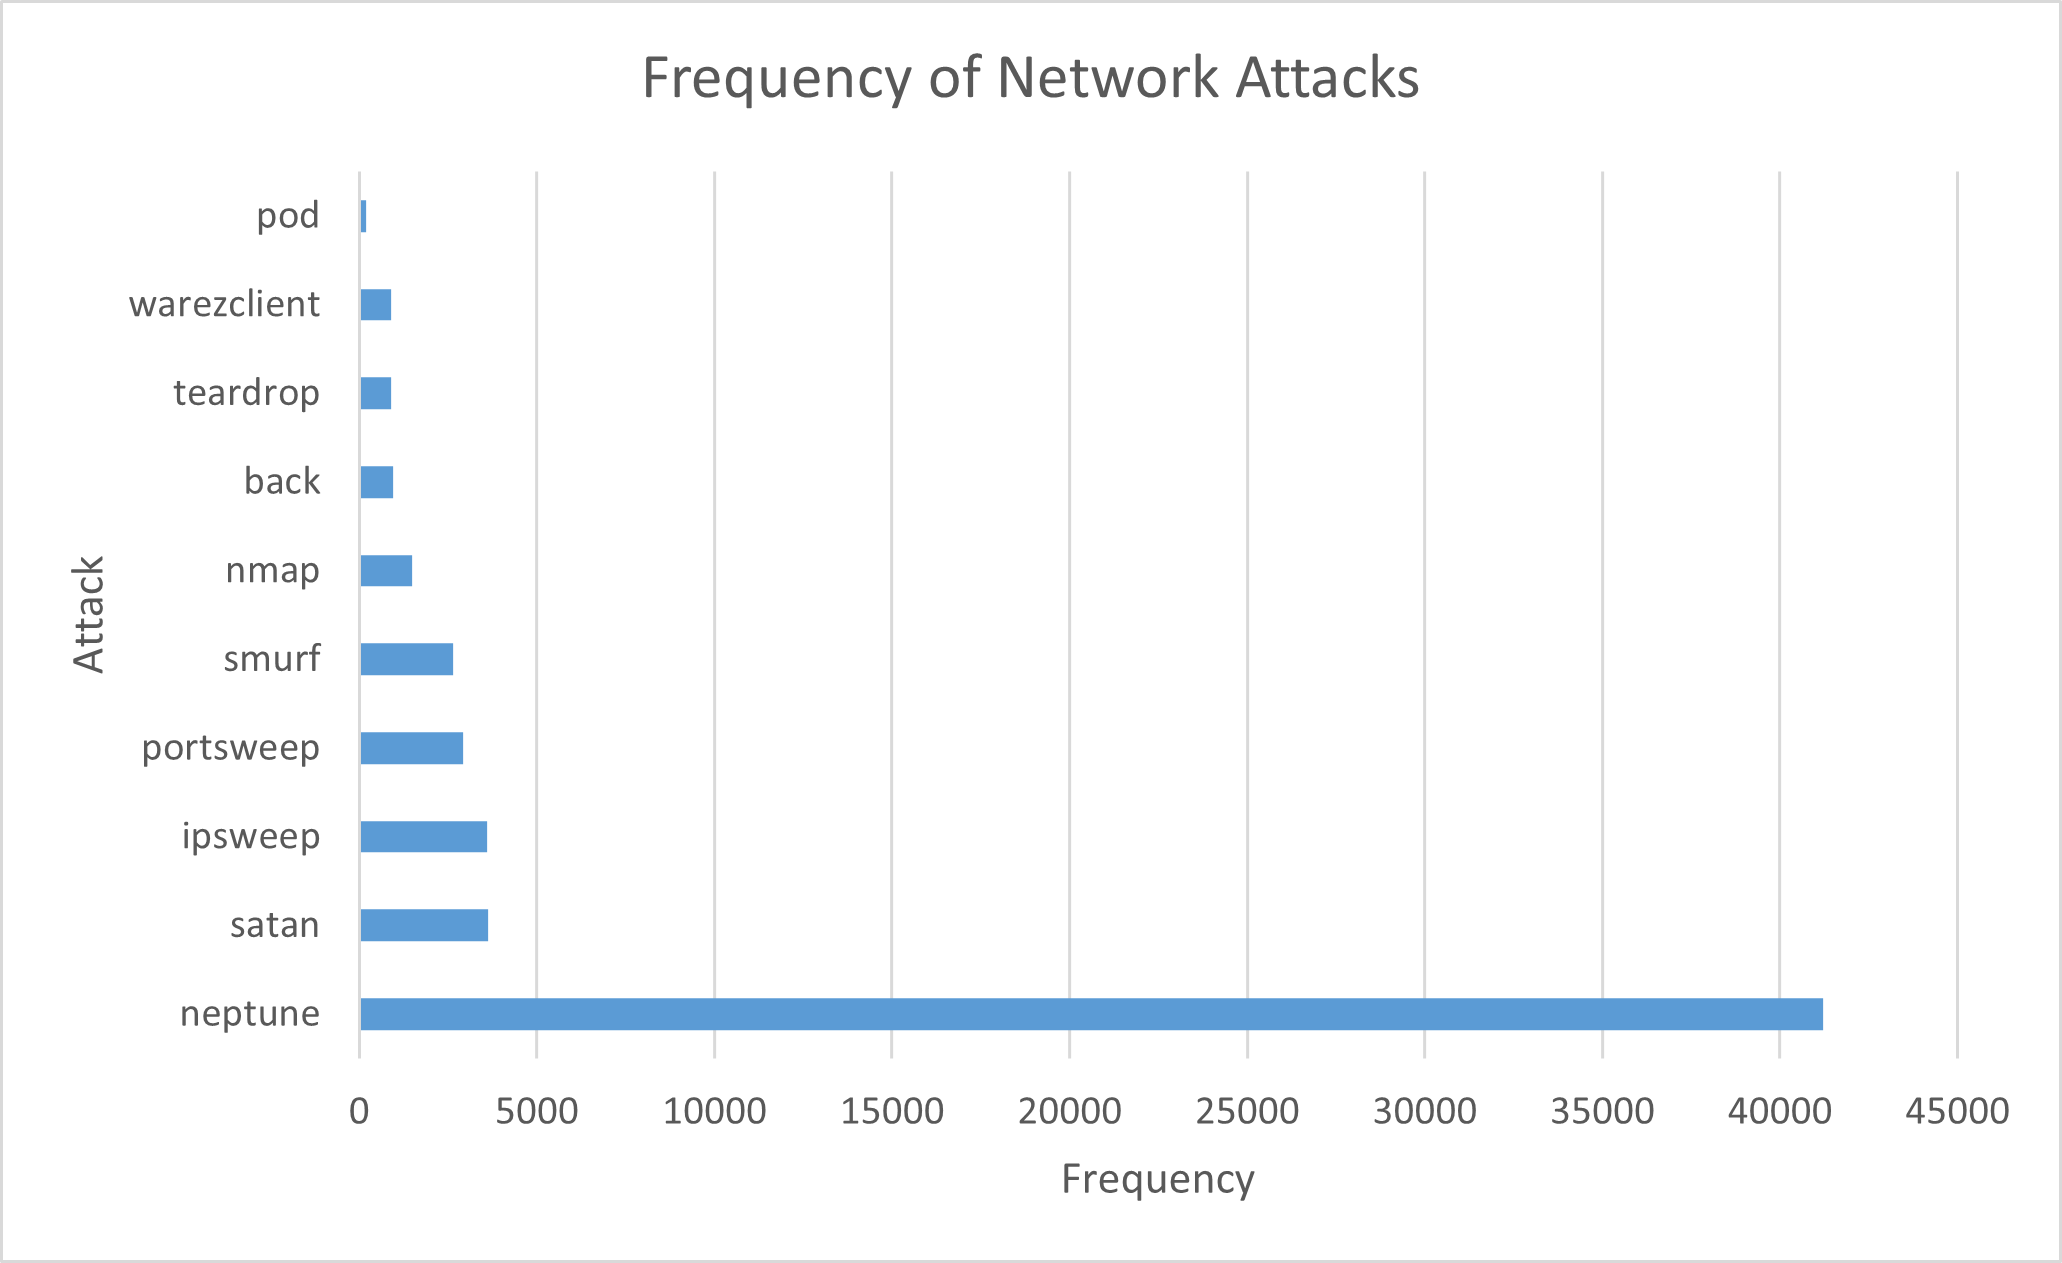
\includegraphics[height= 170 pt, width=0.45\textwidth]{External/Fig-Frequency-of-Attacks.PNG}}
\caption{Top 10 Most Frequent Attacks}
\label{fig1}
\end{figure}

Out of all the data, an intrusion occurred 46.5\% of the time. We further group these attack types into four main types, namely: Denial of Service (DoS), Probe, Privilege and Access attacks. Each type of attack seen in Table \ref{tab1} is classified into one of the four types. The classifications are shown in Table \ref{tab2}. If we look at the number of occurrences of these attacks by type in our dataset as shown in Fig \ref{fig2}, we can see that Denial of Service is the most post popular.

\begin{table}[htbp]
\caption{Frequency of Network Attacks}
\begin{center}
\begin{tabular}{|c|c|c|c|}
\hline
DoS	&	Probe	&	Privilege	&	Access	\\
\hline
apache2	&	ipsweep	&	buffer\_overflow	&	ftp\_write	\\
back	&	mscan	&	loadmodule	&	guess\_passwd	\\
land	&	nmap	&	perl	&	http\_tunnel	\\
neptune	&	portsweep	&	ps	&	imap	\\
mailbomb	&	satan	&	rootkit	&	multihop	\\
pod	&	satan	&	sqlattack	&	named	\\
processtable	&		&	xterm	&	phf	\\
smurf	&		&		&	sendmail	\\
teardrop	&		&		&	snmpgetattack	\\
udpstorm	&		&		&	spy	\\
worm	&		&		&	snmpguess	\\
	&		&		&	warezclient	\\
	&		&		&	warezmaster	\\
	&		&		&	xclock	\\
	&		&		&	xsnoop	\\
\hline
45927 &	 11656  &	 52  &	995
	\\
\hline
\end{tabular}
\label{tab2}
\end{center}
\end{table}

\begin{figure}[htbp]
\centerline{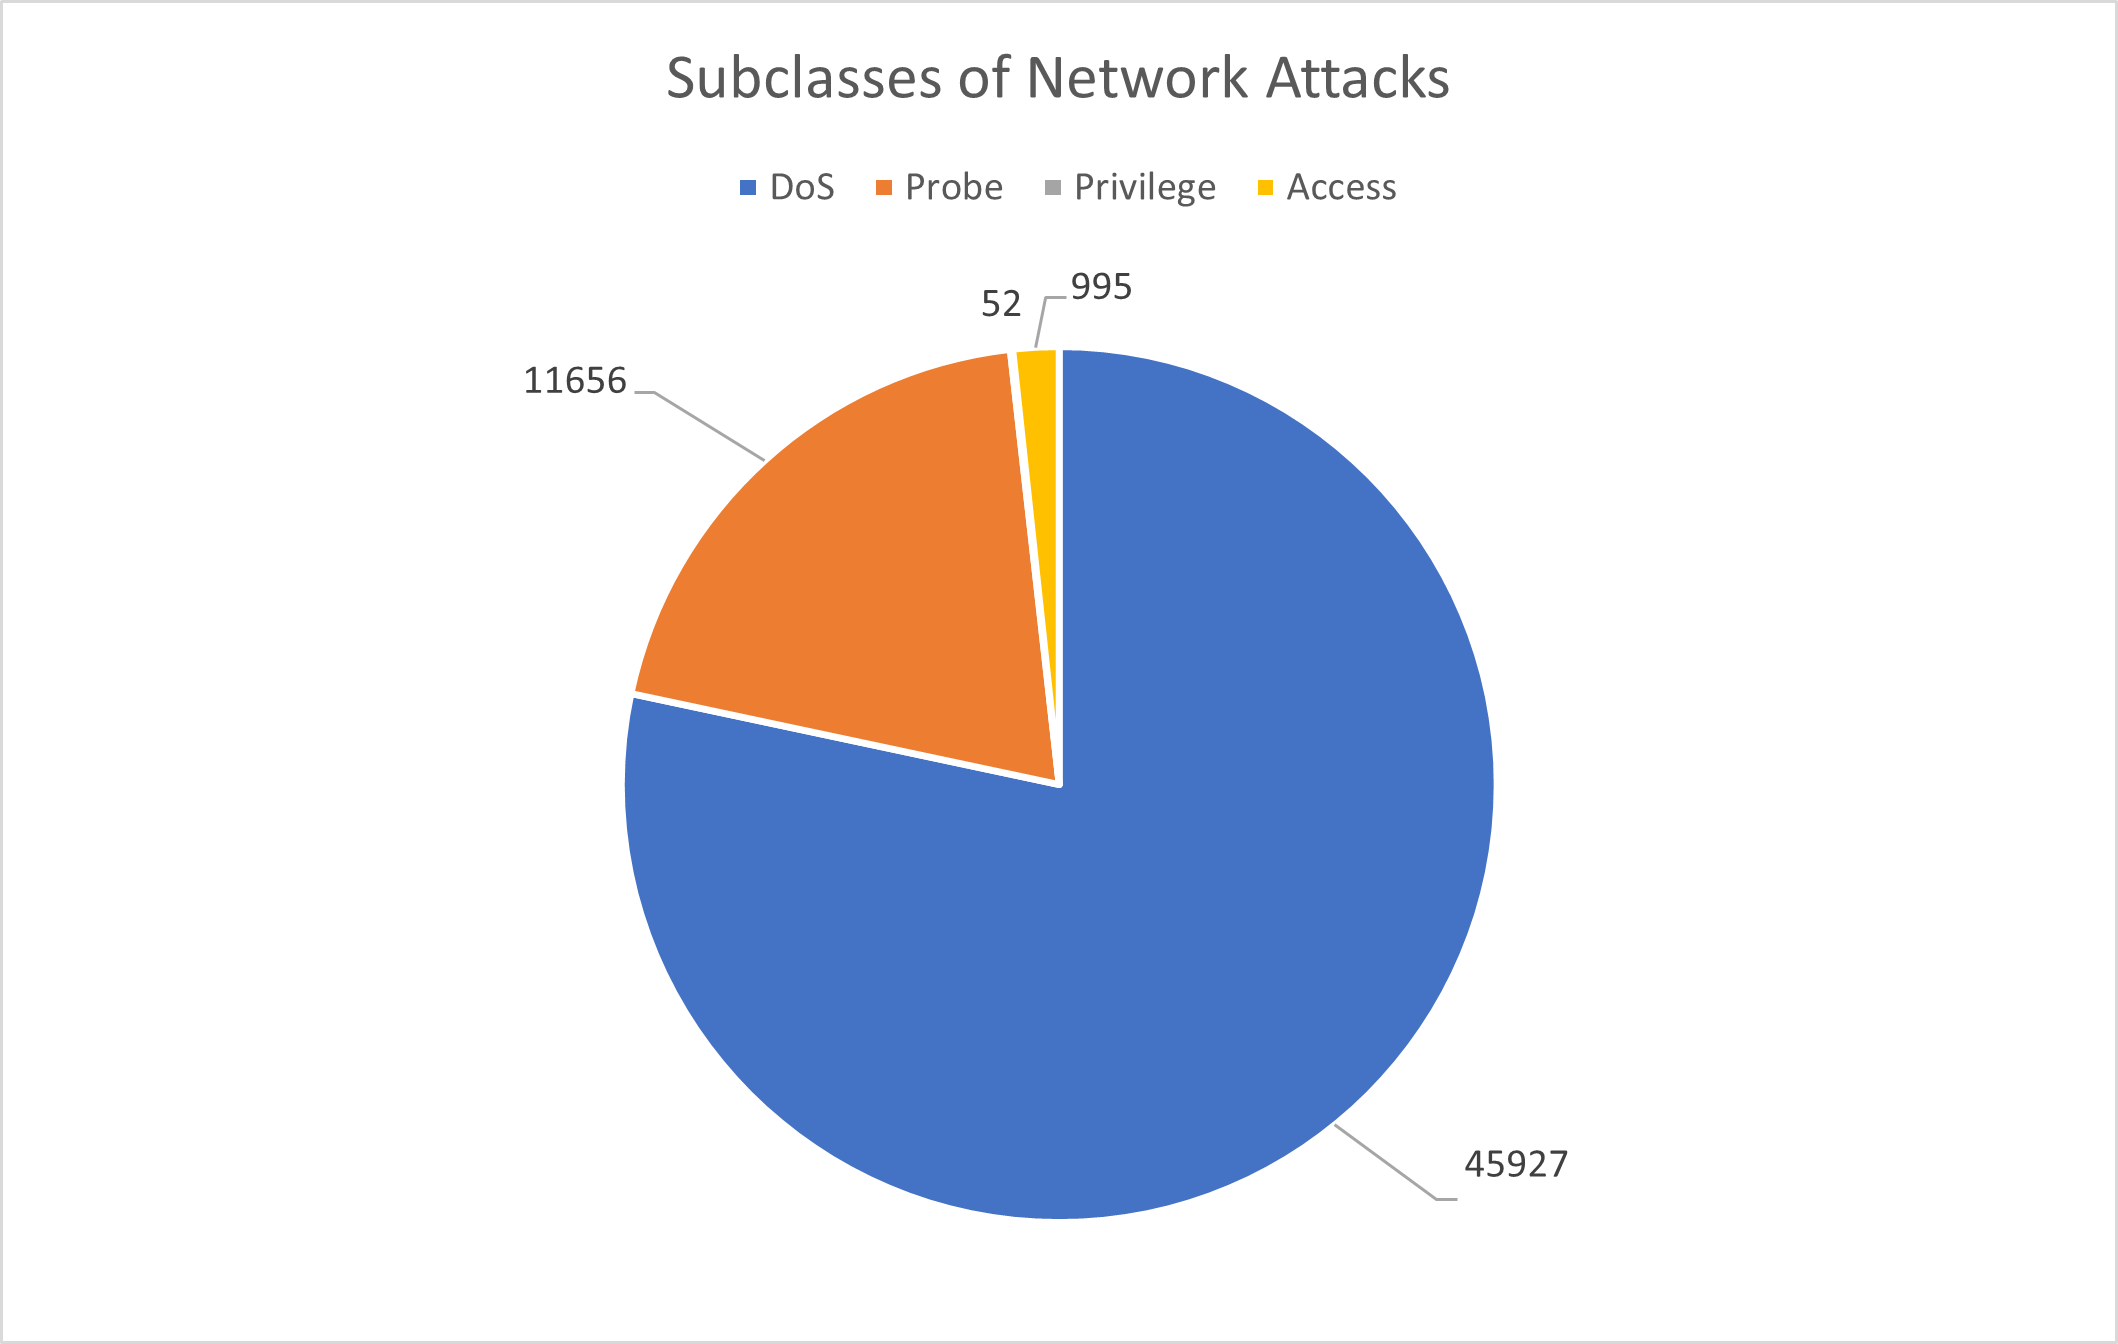
\includegraphics[height= 160 pt, width=0.45\textwidth]{External/Fig-Subclasses-of-Attacks.PNG}}
\caption{Top 10 Most Frequent Attacks}
\label{fig2}
\end{figure}

\section{Data Preprocessing}
For the purpose of our study, we are only interested in detecting the intrusion. That is, we want to find out if any intrusion has occurred in the network system or not. So we approach this problem as a Binary Classification problem. The network system characteristics can denote either \emph{Normal} (No Intrusion detected) or \emph{Intrusion} (Intrusion detected). For this, we encode all \emph{normal} values from \emph{attack} column as \emph{0} which denotes no intrusion and all other \emph{attack} values as \emph{1} which denotes that there has been an intrusion. We add a new column named \emph{is\_intrusion} that will contain the aforementioned flags for each record. The column \emph{is\_intrusion} is now set as our target column.

After specifying the target column, we perform feature selection to find the most relevant fields from the input feature set. As discussed before, we have a total of 42 input features. The feature set contains of both Numeric and Categorical fields. We use a Statistics-based approach to study the relations among the input features and their relationship with the target column. We compute the correlations of the input features with the target column. For this, we encode the categorical variables using one-hot encoding technique. We remove any columns that have a very high ($>0.9$) or a very low ($\sim 0$) correlation with the target column. Then, we select the top 15 features that are most correlated with the target column ordered by their absolute value (to account for both positive and negative correlations). We also perform a co-linearity analysis on the remaining features in order to check if there are any linearly dependent pairs of features.

\section{Implementation}
After the data preprocessing, we reduce the 42 feature sets into 11 selected input features for our model. The features are listed as:
\begin{itemize}
\item flag\_SF: Status of the connection – \emph{SF} denotes normal establishment and termination.
\item same\_srv\_rate: The percentage of connections that were to the same service, among the connections aggregated in \emph{count}.
\item dst\_host\_srv\_count: Number of connections having the same port number.
\item logged\_in: The login status - $1$ if successfully logged in, $0$ otherwise.
\item serror\_rate: The percentage of connections that have activated the \emph{flag} value as $s0, s1, s2$ or $s3$, among the connections aggregated in \emph{count}.
\item count : Number of connections to the same destination host as the current connection in the past two seconds.
\item service\_http : Destination network service used - $http$.
\item service\_private : Destination network service used - $private$.
\item dst\_host\_count: Number of connections having the same destination host IP address.
\item service\_domain\_u: Destination network service used - $domain\_u$.
\item srv\_rerror\_rate: The percentage of connections that have activated the \emph{flag} as \emph{REJ}, among the connections aggregated in \emph{srv\_count}.
\end{itemize}


Since this is a Binary classification problem, we compare the performance of various classifiers and pick the one that performs the best. We compare the performance of Logistic Regression, K Nearest Neighbors and Decision Tree Classifiers. We select Decision Tree Classifier as our benchmark model. Then, we fit the model on the training dataset using a train-test split of 80\% and 20\%. The model gives us a test accuracy of 97.97\% on the train subset. We evaluate the model on the unseen data from test subset, i.e. the KDDTest+ file. 

\section{Results}
The accuracy of predictions of the model was found to be only 77.5\%. This denotes that the model is overfitting on the train subset. This can be mitigated using various techniques like cross-validation, regularization or ensembling. The performance measures reported for the model are shown in Table \ref{tab3}.
\begin{table}[htbp]
\caption{Performance of model}
\begin{center}
\begin{tabular}{|c|c|c|c|}
\hline
Accuracy	&	F1 Score	&	Precision	&	Recall	\\
\hline
0.7745 &	 0.7969  &	 0.8178  &	0.777\\
\hline
\end{tabular}
\label{tab3}
\end{center}
\end{table}

\section{Conclusion}
The goal of this paper was to study various types of attacks that frequently occur in a network system and design a model to identify such intrusions. We evaluated different network parameters that characterize a network system and that help identify networks that are possibly vulnerable to external attacks. We were able to identify the 11 most relevant features out of the 42 input features. The accuracy of the model on the train subset was found to be 97.97\%. However, the model was not able to perform as well on the test subset with an accuracy of only 77.45\%. Thus, the model warrants an improvement to remove the overfitting problem.

\begin{thebibliography}{00}
\bibitem{b1} R. Bace, P. Mell, ``Intrusion detection systems,National Institute of Standards and
Technology (NIST)" , Technical Report, pp. 800-31, 2001.
\bibitem{b2} H. Liao, C. Lin, Y. Lin and K.Tung, ``Intrusion detection system: A comprehensive review", Journal of Network and Computer Applications, vol. 36, pp.16-24, 2013.
\end{thebibliography}

\end{document}
